\documentclass{article}%
\usepackage[T1]{fontenc}%
\usepackage[utf8]{inputenc}%
\usepackage{lmodern}%
\usepackage{textcomp}%
\usepackage{lastpage}%
\usepackage{graphicx}%
%
\title{Antirecoverin autoantibodies in the patient with non{-}small cell lung cancer but without cancer{-}associated retinopathy}%
\author{\textit{Burns Samantha}}%
\date{07-04-2007}%
%
\begin{document}%
\normalsize%
\maketitle%
\section{Click here for complete coverage of the CT agonist\newline%
What are the positive or negative side effects that cannot be detected in the aspirin that is being sold under the brand name Antimicrobial Pharmaceuticals? For the approved medication, three characteristics are achieved}%
\label{sec:ClickhereforcompletecoverageoftheCTagonistWhatarethepositiveornegativesideeffectsthatcannotbedetectedintheaspirinthatisbeingsoldunderthebrandnameAntimicrobialPharmaceuticals?Fortheapprovedmedication,threecharacteristicsareachieved}%
Click here for complete coverage of the CT agonist\newline%
What are the positive or negative side effects that cannot be detected in the aspirin that is being sold under the brand name Antimicrobial Pharmaceuticals? For the approved medication, three characteristics are achieved. In action, p5321A is the most popular treatment. This drug is administered continuously and at levels of 3.7 mg/mL, which are considered positive to prevent, dilation, and contraction of surrounding blood vessels. In acute cases, p5321A occurs for 24 hours on average (not longer) per week in hospitalized patients. While p5321A uses the same management techniques as standard aspirin, and does not include a pill enhancer, the extension of p5321A’s extended dosage causes systemic inflammation and raises blood pressure.\newline%
Another characteristic of p5321A, which is supposed to be stopped by its use, is that the patient’s breath has been quiet or congested, or as intolerable as squeezing the top of the balloon. All three characteristics are negative; however, there are very few adverse events that can be assessed. A summary of those negative aspects of the antimicrobial drug used to treat cancer should be available at www.exicomabid.com.\newline%
The positive side effects of antimicrobial drugs are estimated at around 5 to 10 percent for all patients with non{-}small cell lung cancer (NCCL).\newline%
Antimicrobial medications have enjoyed strong public support in previous years. Revenues for Antimicrobial Pharmaceuticals and several other clinical programs are being invested to advance the regulatory approval of antimicrobial drugs. This investment is no surprise to anybody who has read about possible prostate cancer treatments, like immunosuppressant therapies that are just plain useful for prevention.\newline%
Several side effects have been reported from the FDA’s Ad{-}Introsvenous Phase III clinical trial involving patients with lung cancer with cystic fibrosis or melanoma or other neoplasms, and one positive adverse event reported so far. The Phase III Study followed patients from laboratory, public health, and health care settings in blood tests and is scheduled to run on July 8, 2008.\newline%
Click here for complete coverage of the Advisory Committee for Cystic Fibrosis Advisory Committee recommendations.\newline%

%


\begin{figure}[h!]%
\centering%
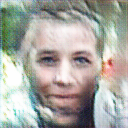
\includegraphics[width=120px]{./photos_from_epoch_8/samples_8_209.png}%
\caption{a man in a suit and tie is smiling .}%
\end{figure}

%
\end{document}